% AUTO-GENERATED by scripts/make_force_traces_pgf.py — do not edit.
% Data: LGES/vla_training/rollouts/smolvla_naive_0729/20260730-142623_ep0000_case_pick (naive) / LGES/vla_training/rollouts/smolvla_film_0729_prefix_mask1/L5/20260730-170039_r03_ep0000_case_pick (FiLM).
\definecolor{figcond}{HTML}{0072B2}
\definecolor{fignaive}{HTML}{D55E00}
\definecolor{figmuted}{HTML}{767676}
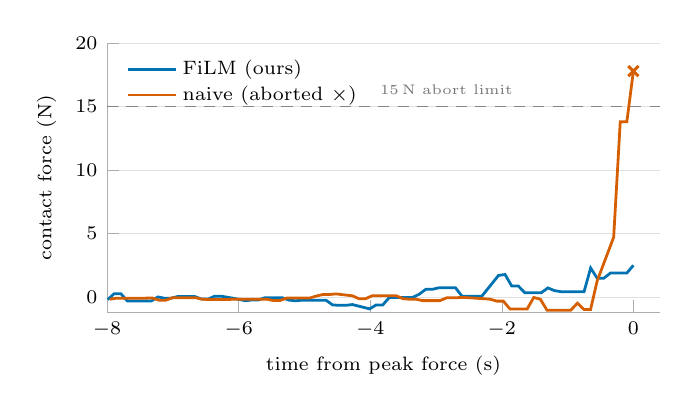
\begin{tikzpicture}
\begin{axis}[
  width=8.6cm, height=5.0cm, xmin=-8, xmax=0.4, ymin=-1.2, ymax=20,
  xtick={-8,-6,-4,-2,0}, ytick={0,5,10,15,20},
  xlabel={time from peak force (s)}, ylabel={contact force (N)},
  tick label style={font=\scriptsize}, label style={font=\scriptsize},
  axis x line*=bottom, axis y line*=left,
  axis line style={figmuted!60, line width=0.4pt},
  tick style={figmuted!60},
  ymajorgrids, grid style={figmuted!22, line width=0.3pt},
  clip=false, legend style={draw=none, fill=none, font=\scriptsize,
    legend cell align=left, at={(0.02,0.98)}, anchor=north west, row sep=-1.5pt},
]
\addplot[figmuted!90, dash pattern=on 4pt off 3pt, line width=0.5pt, forget plot] coordinates {(-8,15) (0.4,15)};
\node[font=\tiny, figmuted, anchor=south west] at (axis cs:-4.0,15.2) {15\,N abort limit};
\addplot[figcond, line width=1.0pt] coordinates {(-7.992,-0.20) (-7.892,0.27) (-7.792,0.27) (-7.692,-0.31) (-7.592,-0.31) (-7.328,-0.31) (-7.228,0.01) (-7.128,-0.09) (-7.028,-0.09) (-6.928,0.04) (-6.665,0.04) (-6.565,-0.16) (-6.465,-0.16) (-6.365,0.07) (-6.265,0.07) (-6.001,-0.17) (-5.901,-0.29) (-5.801,-0.23) (-5.701,-0.23) (-5.601,-0.05) (-5.337,-0.05) (-5.237,-0.24) (-5.137,-0.29) (-5.037,-0.25) (-4.937,-0.25) (-4.672,-0.25) (-4.572,-0.62) (-4.472,-0.65) (-4.372,-0.65) (-4.272,-0.59) (-4.010,-0.93) (-3.910,-0.62) (-3.810,-0.62) (-3.710,-0.03) (-3.610,-0.03) (-3.357,-0.03) (-3.257,0.22) (-3.157,0.61) (-3.057,0.61) (-2.957,0.73) (-2.704,0.73) (-2.604,0.06) (-2.504,0.06) (-2.404,0.07) (-2.304,0.07) (-2.051,1.70) (-1.951,1.78) (-1.851,0.88) (-1.751,0.88) (-1.651,0.34) (-1.400,0.34) (-1.300,0.72) (-1.200,0.51) (-1.100,0.42) (-1.000,0.42) (-0.750,0.42) (-0.650,2.29) (-0.550,1.48) (-0.450,1.48) (-0.350,1.89) (-0.100,1.89) (0.000,2.50)};
\addlegendentry{FiLM (ours)}
\addplot[fignaive, line width=1.0pt] coordinates {(-7.959,-0.17) (-7.859,-0.09) (-7.759,-0.10) (-7.659,-0.10) (-7.559,-0.09) (-7.309,-0.08) (-7.209,-0.25) (-7.109,-0.25) (-7.009,-0.05) (-6.909,-0.05) (-6.657,-0.05) (-6.557,-0.17) (-6.457,-0.19) (-6.357,-0.19) (-5.820,-0.17) (-5.571,-0.17) (-5.471,-0.27) (-5.371,-0.27) (-5.271,-0.08) (-5.171,-0.08) (-4.921,-0.08) (-4.821,0.08) (-4.721,0.20) (-4.621,0.20) (-4.521,0.25) (-4.272,0.10) (-4.172,-0.13) (-4.072,-0.13) (-3.972,0.10) (-3.872,0.10) (-3.603,0.10) (-3.503,-0.13) (-3.403,-0.17) (-3.303,-0.17) (-3.203,-0.28) (-2.940,-0.28) (-2.839,-0.06) (-2.739,-0.06) (-2.639,-0.04) (-2.539,-0.04) (-2.276,-0.13) (-2.176,-0.17) (-2.076,-0.32) (-1.976,-0.32) (-1.876,-0.94) (-1.615,-0.94) (-1.515,-0.03) (-1.414,-0.17) (-1.314,-1.03) (-1.214,-1.03) (-0.951,-1.03) (-0.851,-0.48) (-0.751,-0.98) (-0.651,-0.98) (-0.551,1.27) (-0.300,4.71) (-0.200,13.80) (-0.100,13.80) (0.000,17.80)};
\addlegendentry{naive (aborted $\times$)}
\addplot[only marks, mark=x, mark size=2.6pt, fignaive, line width=1.1pt, forget plot] coordinates {(0.000,17.80)};
\end{axis}
\end{tikzpicture}
